\appendix

\section{Apêndice}

% - - - - - - - - - - - - - - - - - - - - - - - - - - -

\subsection{Manual do utilizador}

% - - - - - - - - - - - - - - - - - - - - - - - - - - -

\subsubsection{Execução da plataforma}

\textit{As instruções apresentadas de seguida assumem que o ambiente de desenvolvimento é uma distribuição Linux.}

\bigskip

A plataforma foi feita com a framework de PHP \href{https://laravel.com/}{Laravel}, portanto a primeira coisa a fazer é instalar o \href{https://getcomposer.org/}{Composer}.

\bigskip

O próximo passo é descarregar o projeto, navegar até à pasta \texttt{coexpr}, e instalar as dependências com o comando:

\smallskip

\texttt{composer install}

\bigskip

De seguida, é preciso criar o ficheiro de ambiente \textit{.env}, e gerar uma chave para a aplicação. Para isso, é necessário correr os seguintes comandos:

\smallskip

\texttt{cp .env.example .env}

\texttt{php artisan key:generate}

\medskip

\begin{figure}[ht]
    \centering
    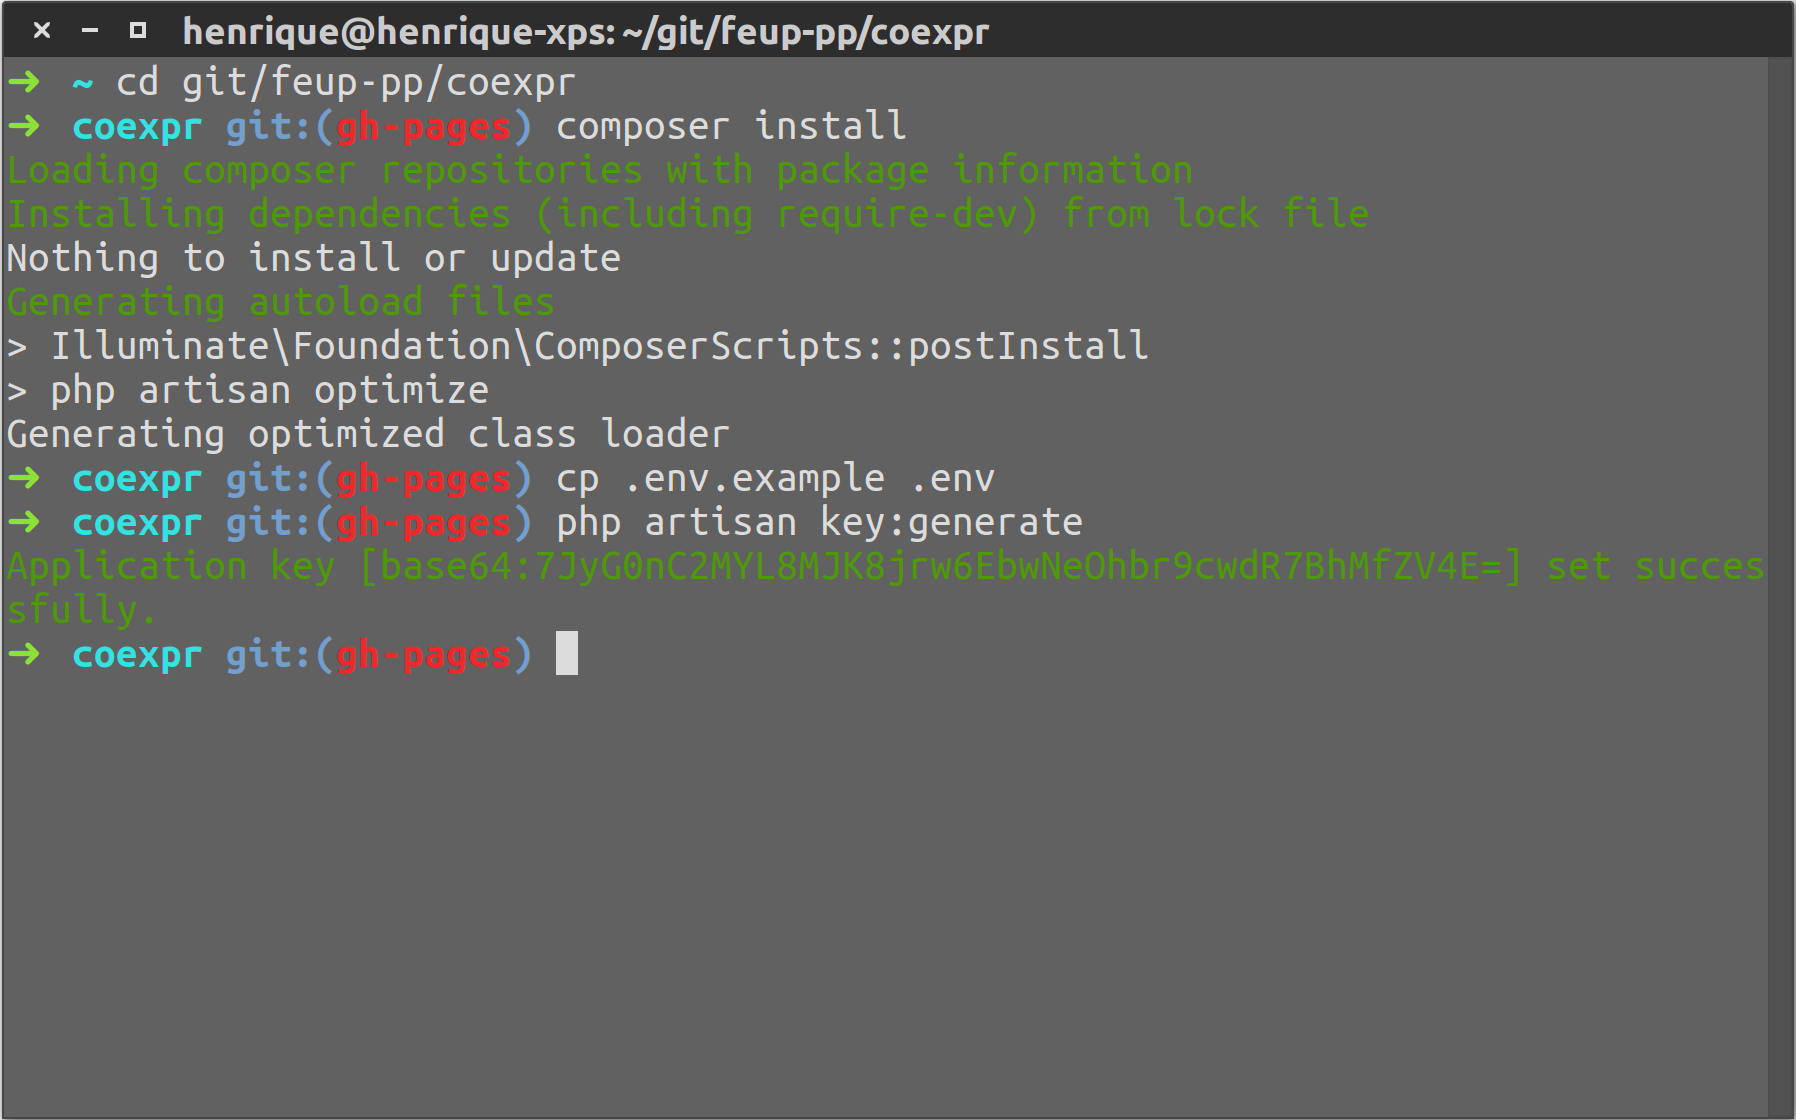
\includegraphics[width=1\linewidth]{res/install-proj.png}
    \caption{Screenshot da instalação do projeto através do terminal.}
\end{figure}

\medskip

Finalmente, para lançar a plataforma basta correr o seguinte comando:

\smallskip

\texttt{php artisan serve}

\bigskip

Depois do comando anterior, ao navegar até \url{http://localhost:8000/}, o utilizador deverá conseguir ver a página principal da plataforma - tal como na figura \ref{fig:homePage}.

Para terminar a execução local da plataforma, basta voltar ao terminal e interromper o comando pressionando as teclas \keys{\ctrl + C}.

% - - - - - - - - - - - - - - - - - - - - - - - - - - -

\subsubsection{Preparação da base de dados}

\textit{Ao explorar um tecido na plataforma, a tabela desse tecido encontra-se vazia. Isso deve-se ao facto de a plataforma já estar operacional, mas a base de dados se encontrar vazia.}

\textit{Esta secção serve para preparar a base de dados, para que possa então ser consultada através da plataforma.}

\bigskip

A primeira coisa a fazer é descarregar o \href{http://www.gtexportal.org/static/datasets/gtex_analysis_v6/rna_seq_data/GTEx_Analysis_v6_RNA-seq_RNA-SeQCv1.1.8_gene_rpkm.gct.gz}{ficheiro comprimido} que contém toda a informação genética de que a plataforma precisa.

Assumindo, deste ponto em diante, que a estrutura de ficheiros do projeto é igual à da figura \ref{fig:projectTree}, o próximo passo é descompactar o ficheiro descarregado na pasta \directory{project/data/input/rna-seq-data/}.

\medskip

\begin{figure}[ht]
    \centering
    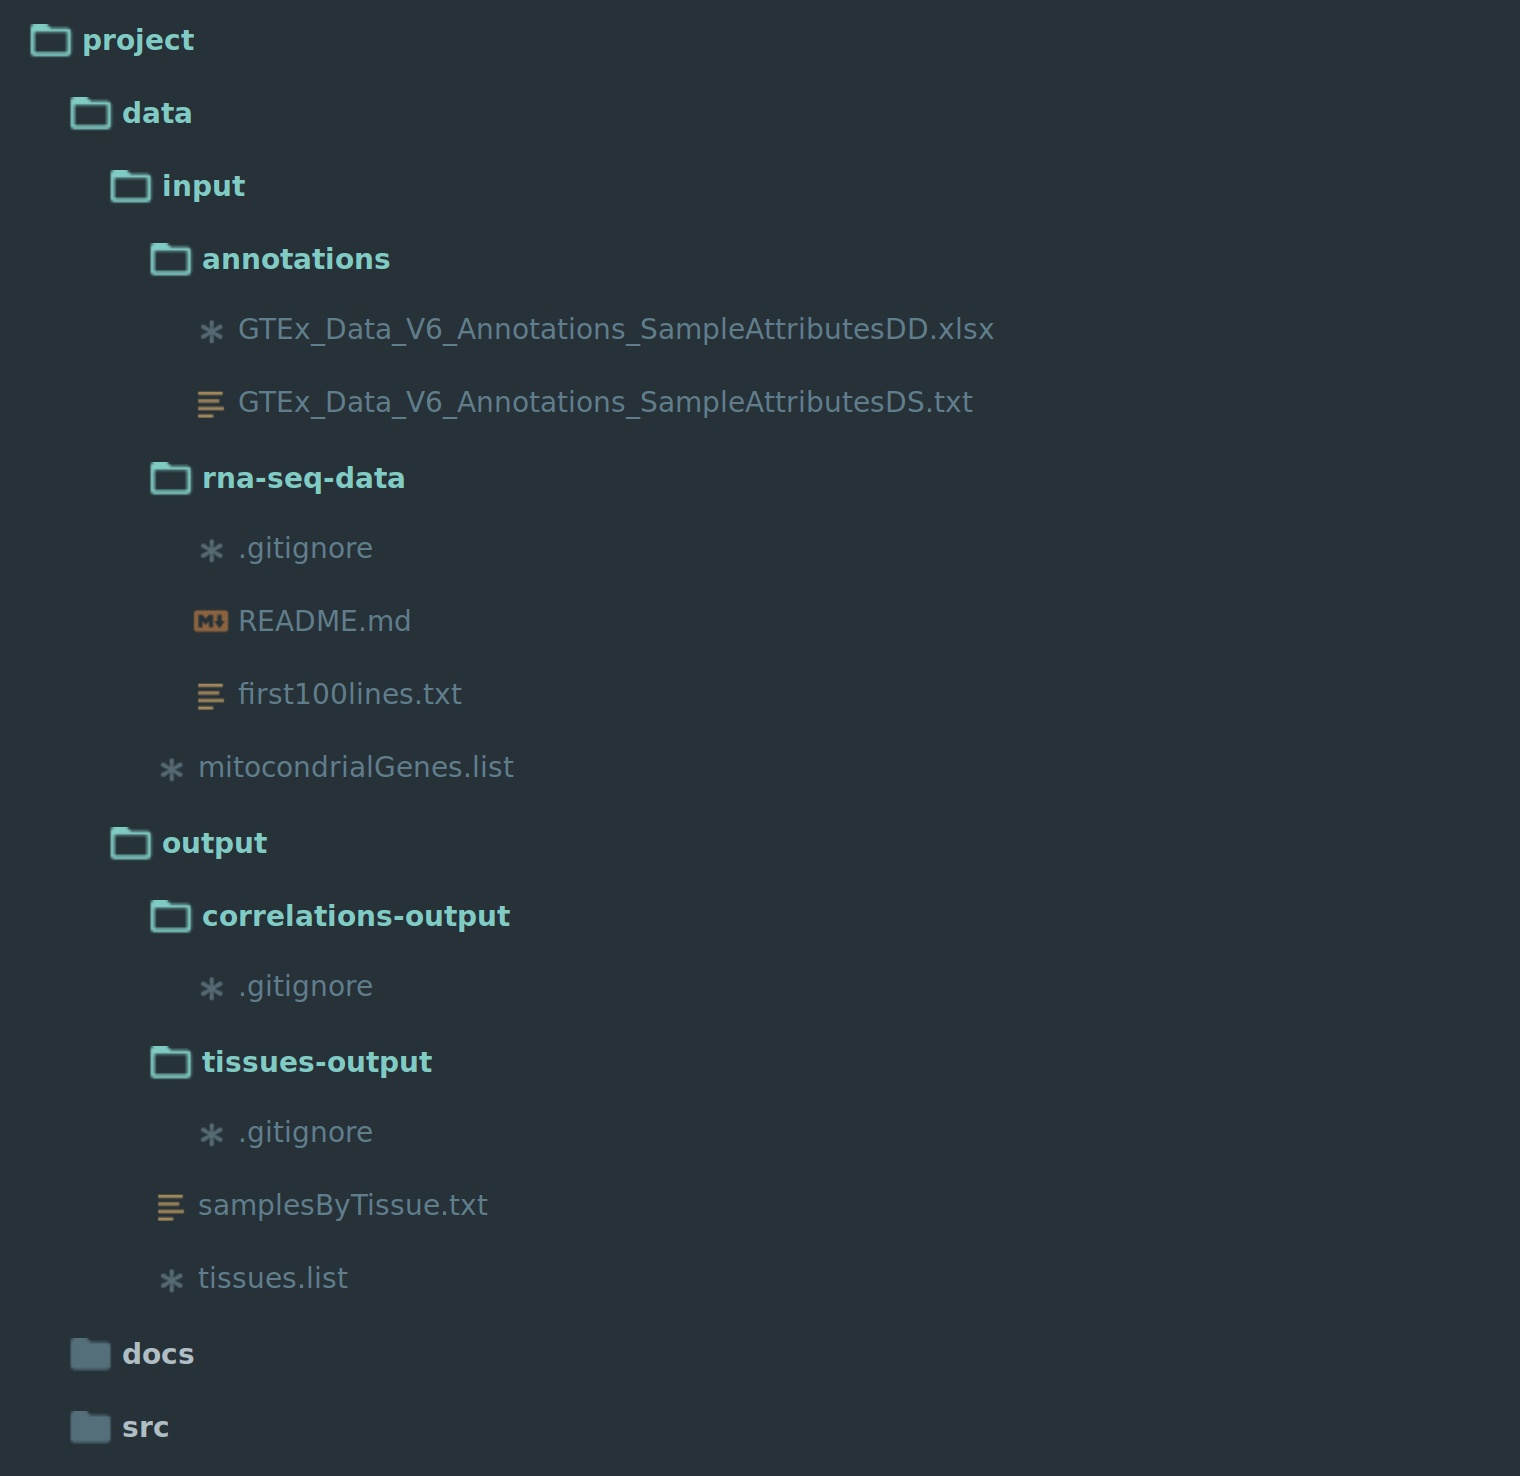
\includegraphics[width=0.7\linewidth]{res/project-tree.png}
    \caption{Estrutura de ficheiros do projeto que usa \textit{C++} para preparar e preencher a base de dados que é utilizada pela plataforma.}
    \label{fig:projectTree}
\end{figure}

\medskip

Depois de o ficheiro descompactado ser colocado na pasta \texttt{rna-seq-data}, o passo seguinte é, através do terminal, navegar atá à pasta \directory{project/src/} e correr os seguintes comandos:

\smallskip

\texttt{g++ parser.cpp -o parser.out -Wall -std=c++11}

\smallskip

\texttt{\seqsplit{./parser.out\ ../data/input/rna-seq-data/All\_Tissue\_Site\_Details\_Analysis.combined.rpkm.gct\ ../data/input/annotations/GTEx\_Data\_V6\_Annotations\_SampleAttributesDS.txt}}

\medskip

\begin{figure}[ht]
    \centering
    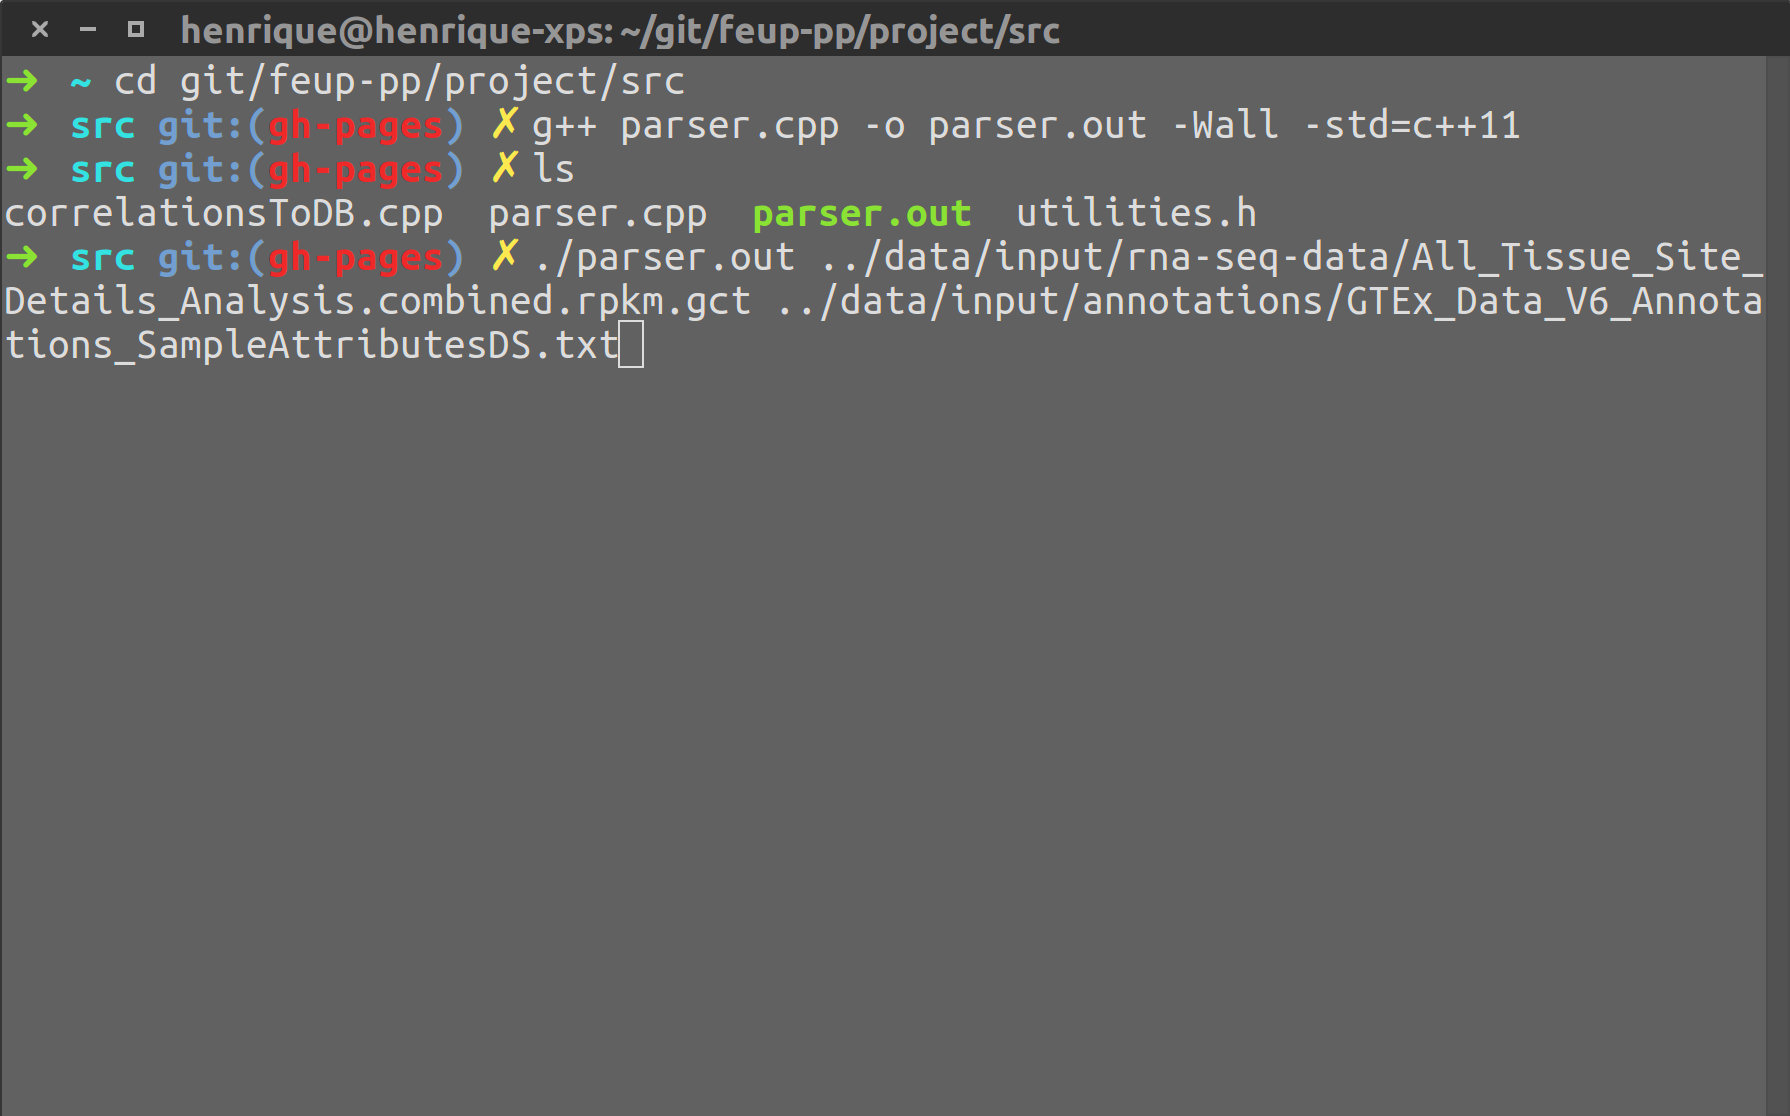
\includegraphics[width=0.7\linewidth]{res/parser-1.png}
    \caption{Execução dos dois comandos acima apresentados.}
    \label{fig:parser-1}
\end{figure}

\medskip

\begin{figure}[ht]
    \centering
    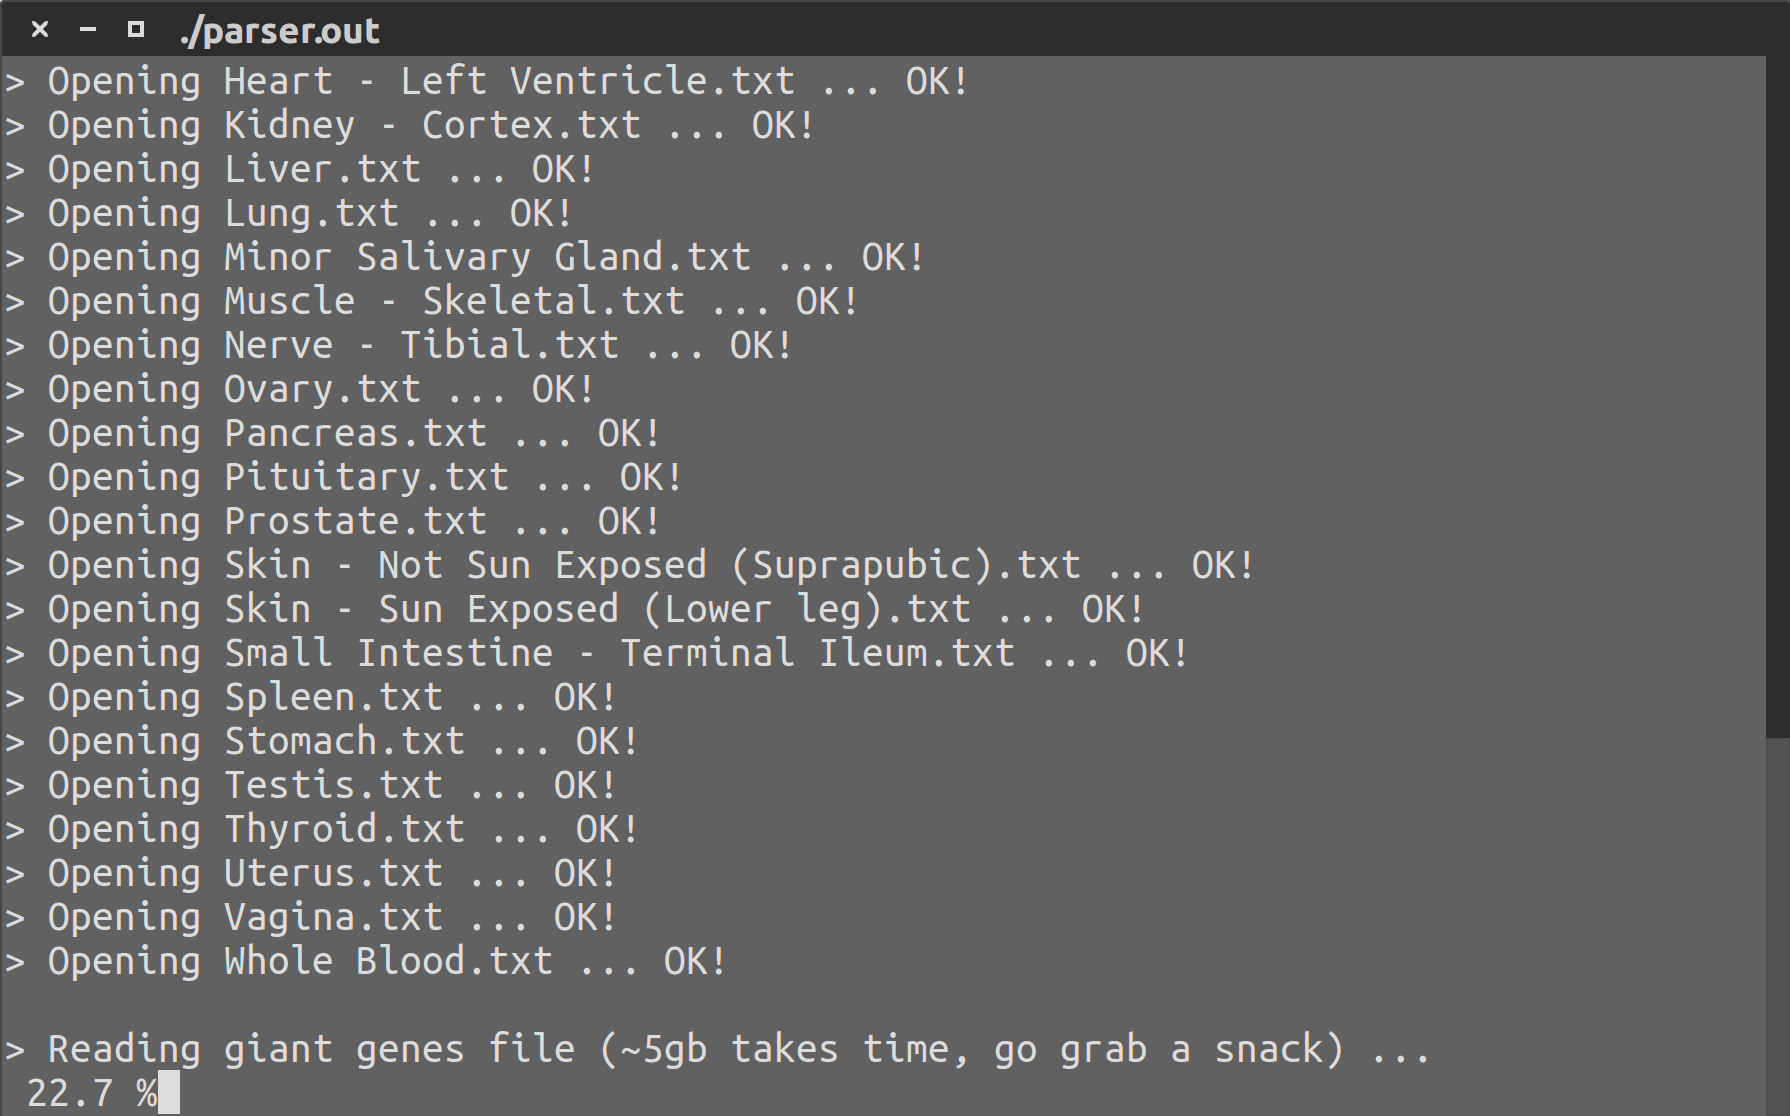
\includegraphics[width=0.7\linewidth]{res/parser-2.png}
    \caption{Output da execução do \textit{parser} sobre o ficheiro descompactado. Este programa demora alguns minutos até terminar.}
    \label{fig:parser-2}
\end{figure}

\medskip

Após correr o \textit{parser}, é necessário fazer \texttt{touch} às bases de dados. Para isso, basta correr o script \textit{refreshDBs.sh}, e executar um comando adicional para criar as tabelas necessárias em cada base de dados:

\smallskip

\texttt{sh refreshDBs.sh}

\smallskip

\texttt{php artisan migrate:refresh}

\medskip

\begin{figure}[ht]
    \centering
    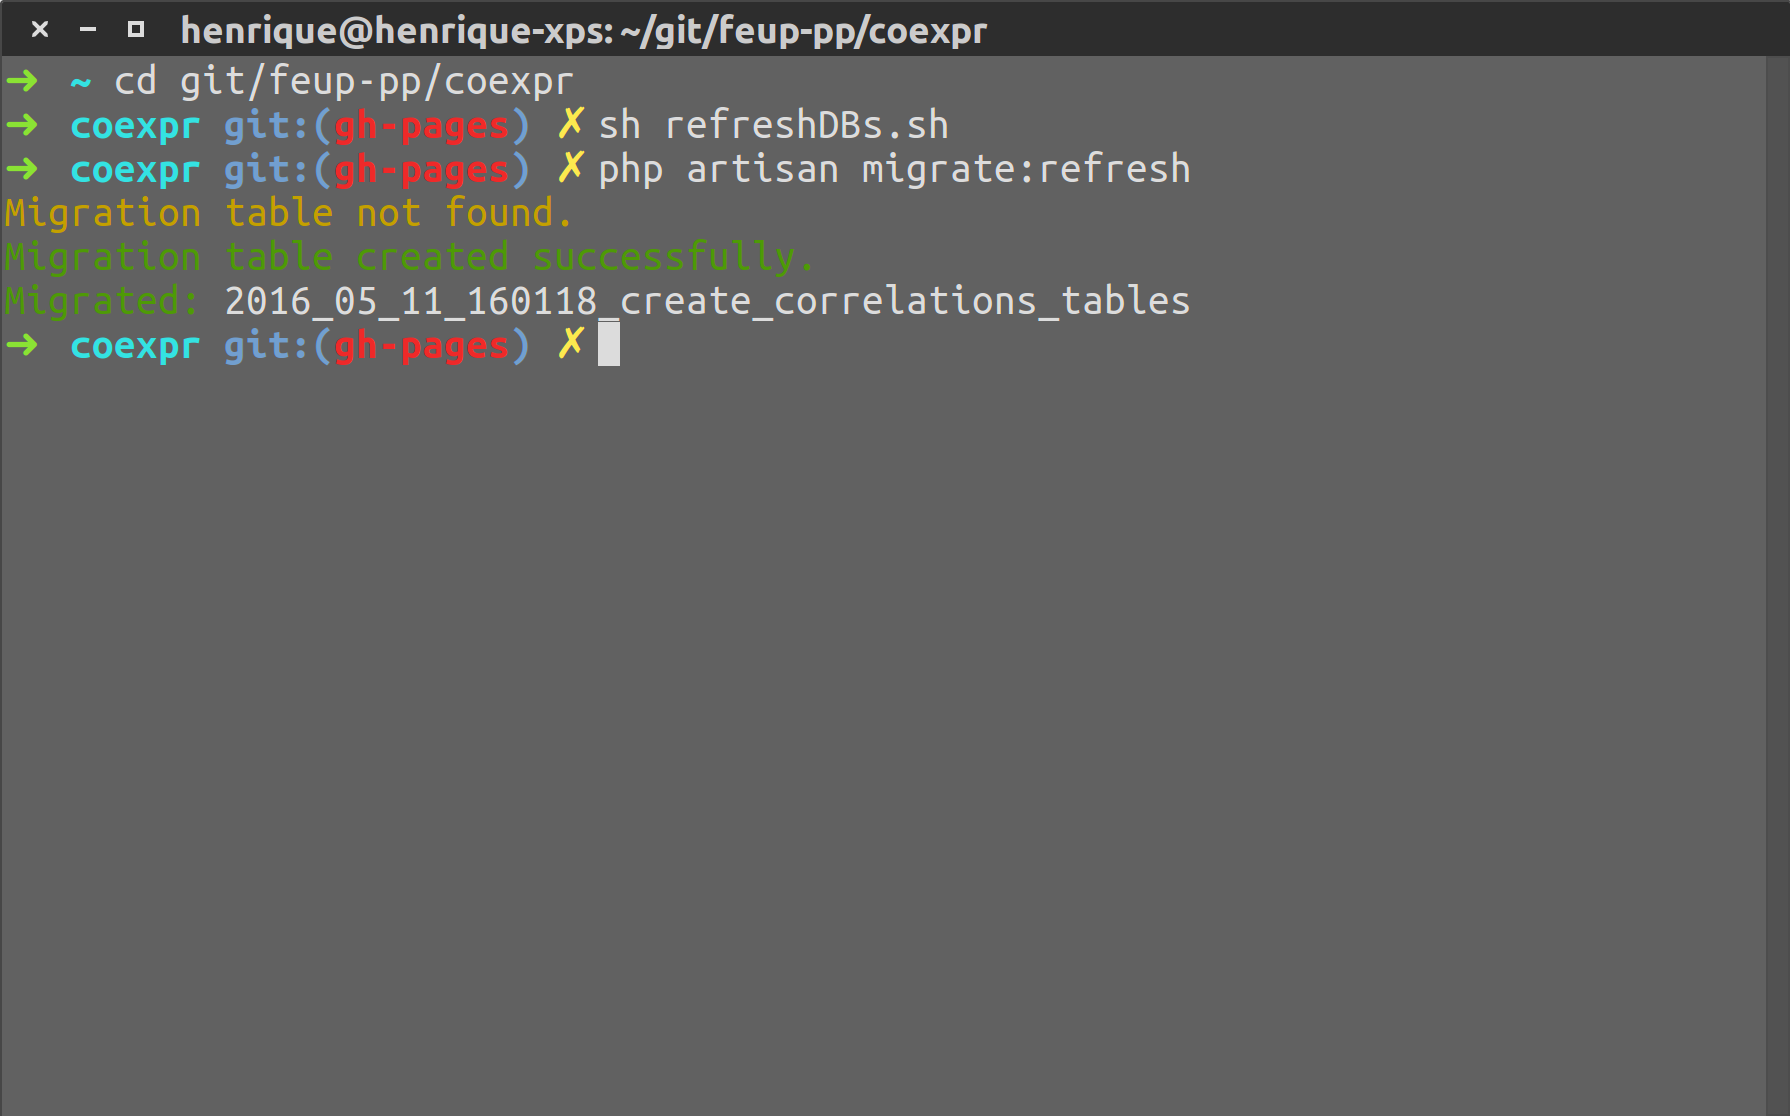
\includegraphics[width=0.7\linewidth]{res/touch-dbs.png}
    \caption{Instância de um terminal onde se fez \textit{refresh} às bases de dados. Após estes comandos, as bases de dados encontram-se inicializadas, mas vazias.}
    \label{fig:touch-db}
\end{figure}

\medskip

Depois disto, as bases de dados já estão prontas para serem preenchidas. Finalmente, para as preencher, é preciso compilar e correr o programa \textit{correlationsToDB} para cada tecido.

\smallskip

\texttt{\seqsplit{g++\ correlationsToDB.cpp\ -o\ correlationsToDB.out\ -Wall\ -lsqlite3\ -std=c++11}}

\smallskip

\texttt{\seqsplit{./correlationsToDB.out\ "Bladder"\ ../data/input/mitocondrialGenes.list}}

\medskip

\begin{figure}[ht]
    \centering
    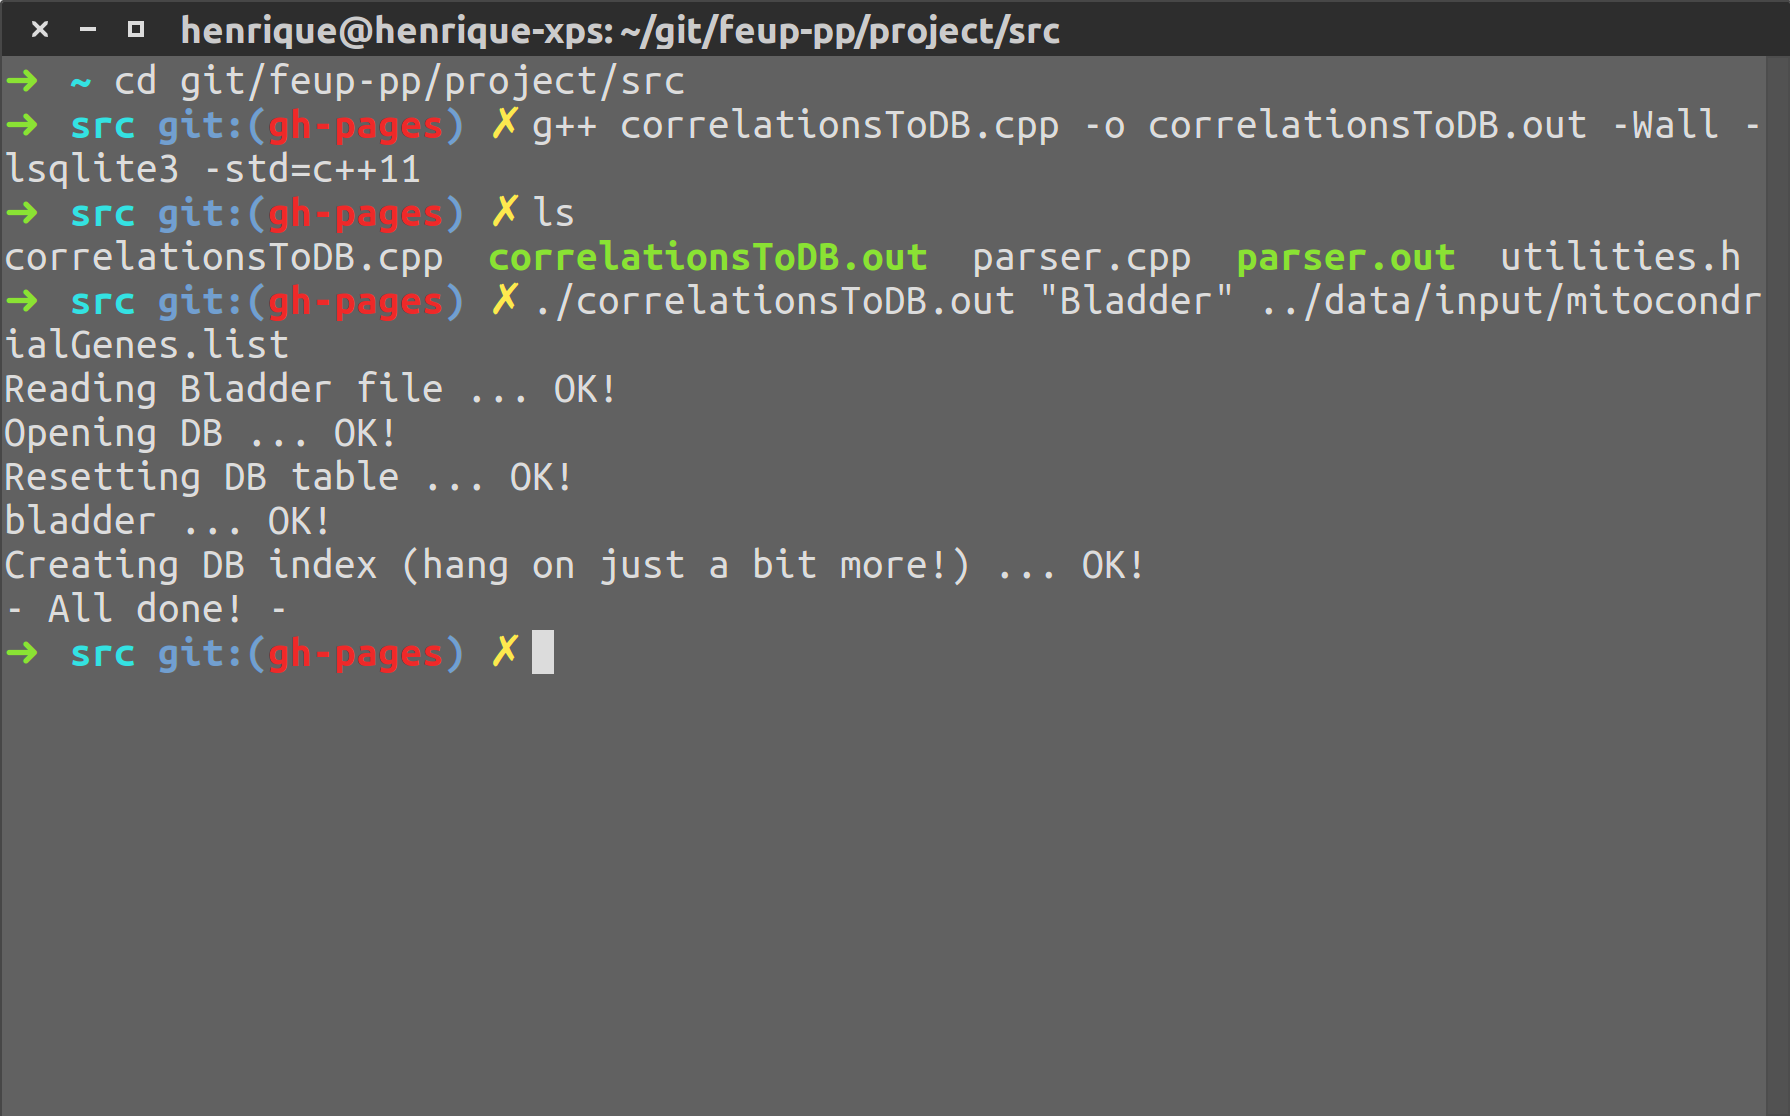
\includegraphics[width=0.7\linewidth]{res/build-tissue-db.png}
    \caption{Resultado da compilação do programa \textit{correlationsToDB}, e da execução do mesmo para o tecido \textit{Bladder}.}
    \label{fig:build-tissue-db}
\end{figure}

\medskip

Neste exemplo, após a execução dos comandos acima, o tecido \textit{Bladder} está pronto para ser consultado através da plataforma. Se o utilizador navegar até à página do tecido, a tabela já deverá ter a informação disponível, tal como é exemplificado na figura \ref{fig:tissuePage}.

\newpage

% - - - - - - - - - - - - - - - - - - - - - - - - - - -

\subsection{Screenshots da plataforma}

\begin{figure}[ht]
    \centering
    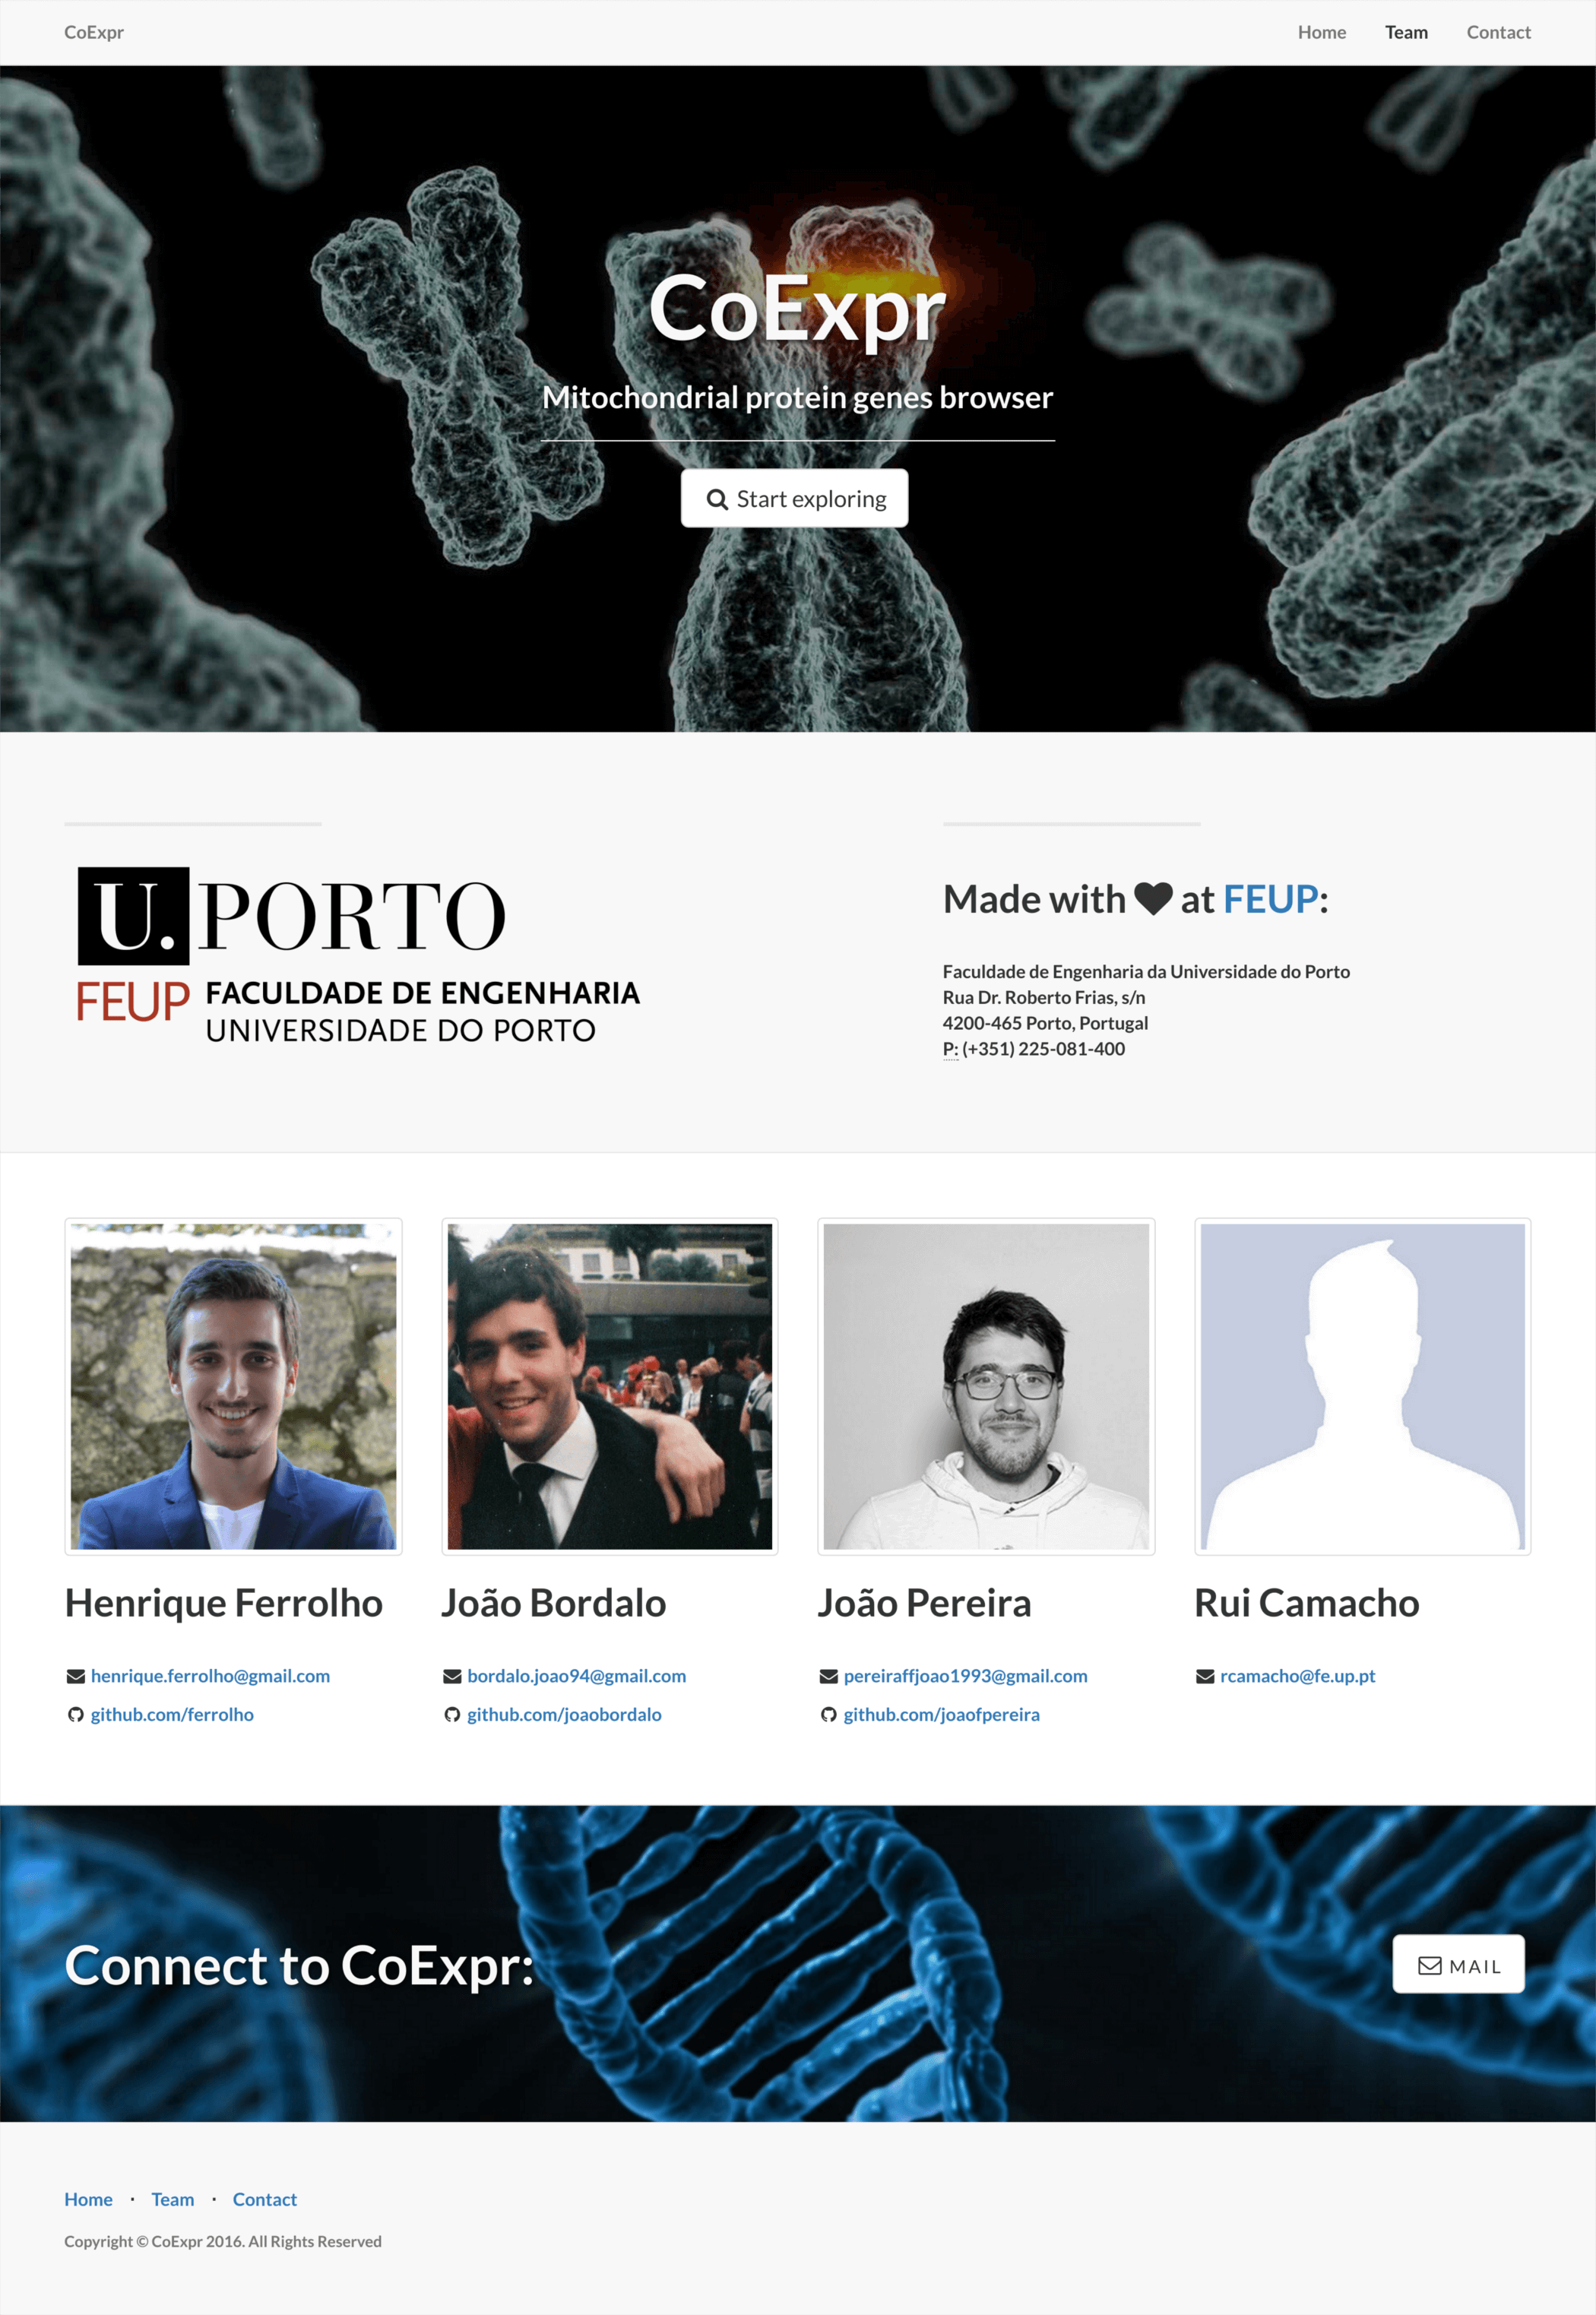
\includegraphics[width=0.7\linewidth]{res/home.png}
    \caption{Página principal da plataforma online. O botão \textit{Start exploring}, no topo, encaminha o utilizador para a página de seleção do tecido a explorar - figura \ref{fig:tissueSelection}.}
    \label{fig:homePage}
\end{figure}

\begin{figure}[ht]
    \centering
    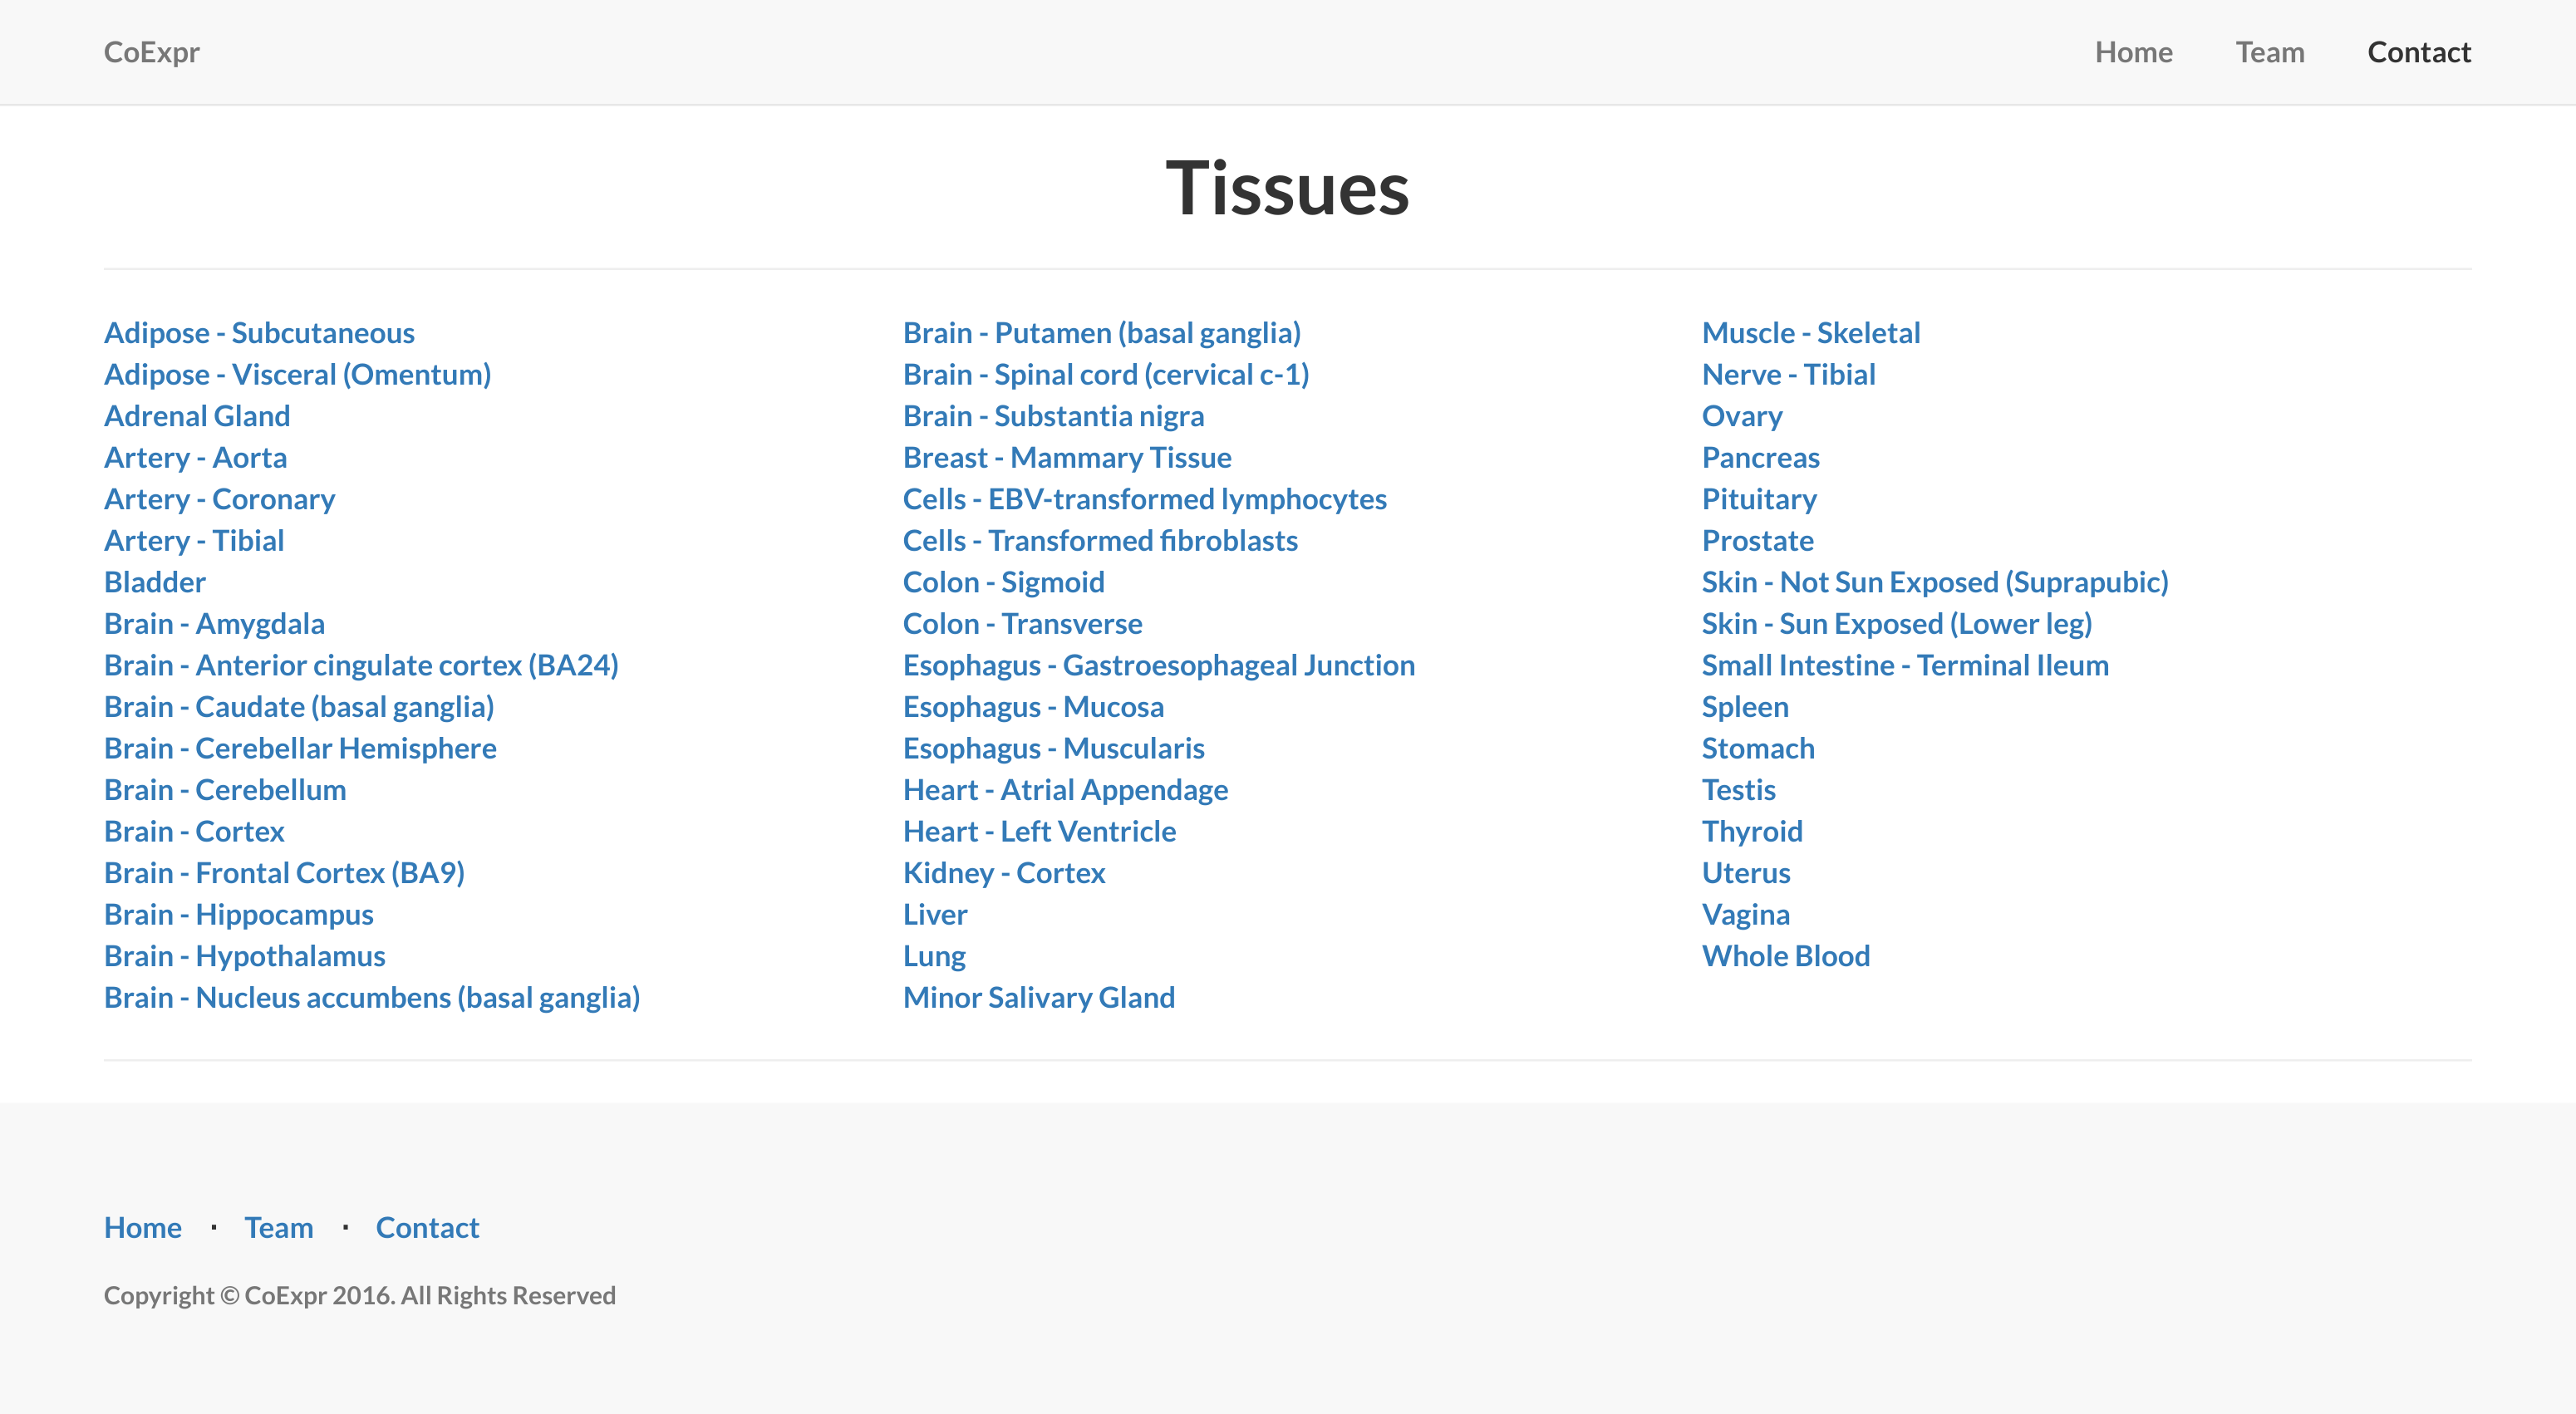
\includegraphics[width=1\linewidth]{res/tissues.png}
    \caption{Página com a lista de tecidos disponíveis a serem explorados. Quando o utilizador carrega num dos tecidos, é encaminhado para a página específica de pesquisa nesse tecido - figura \ref{fig:tissuePage}.}
    \label{fig:tissueSelection}
\end{figure}

\begin{figure}[ht]
    \centering
    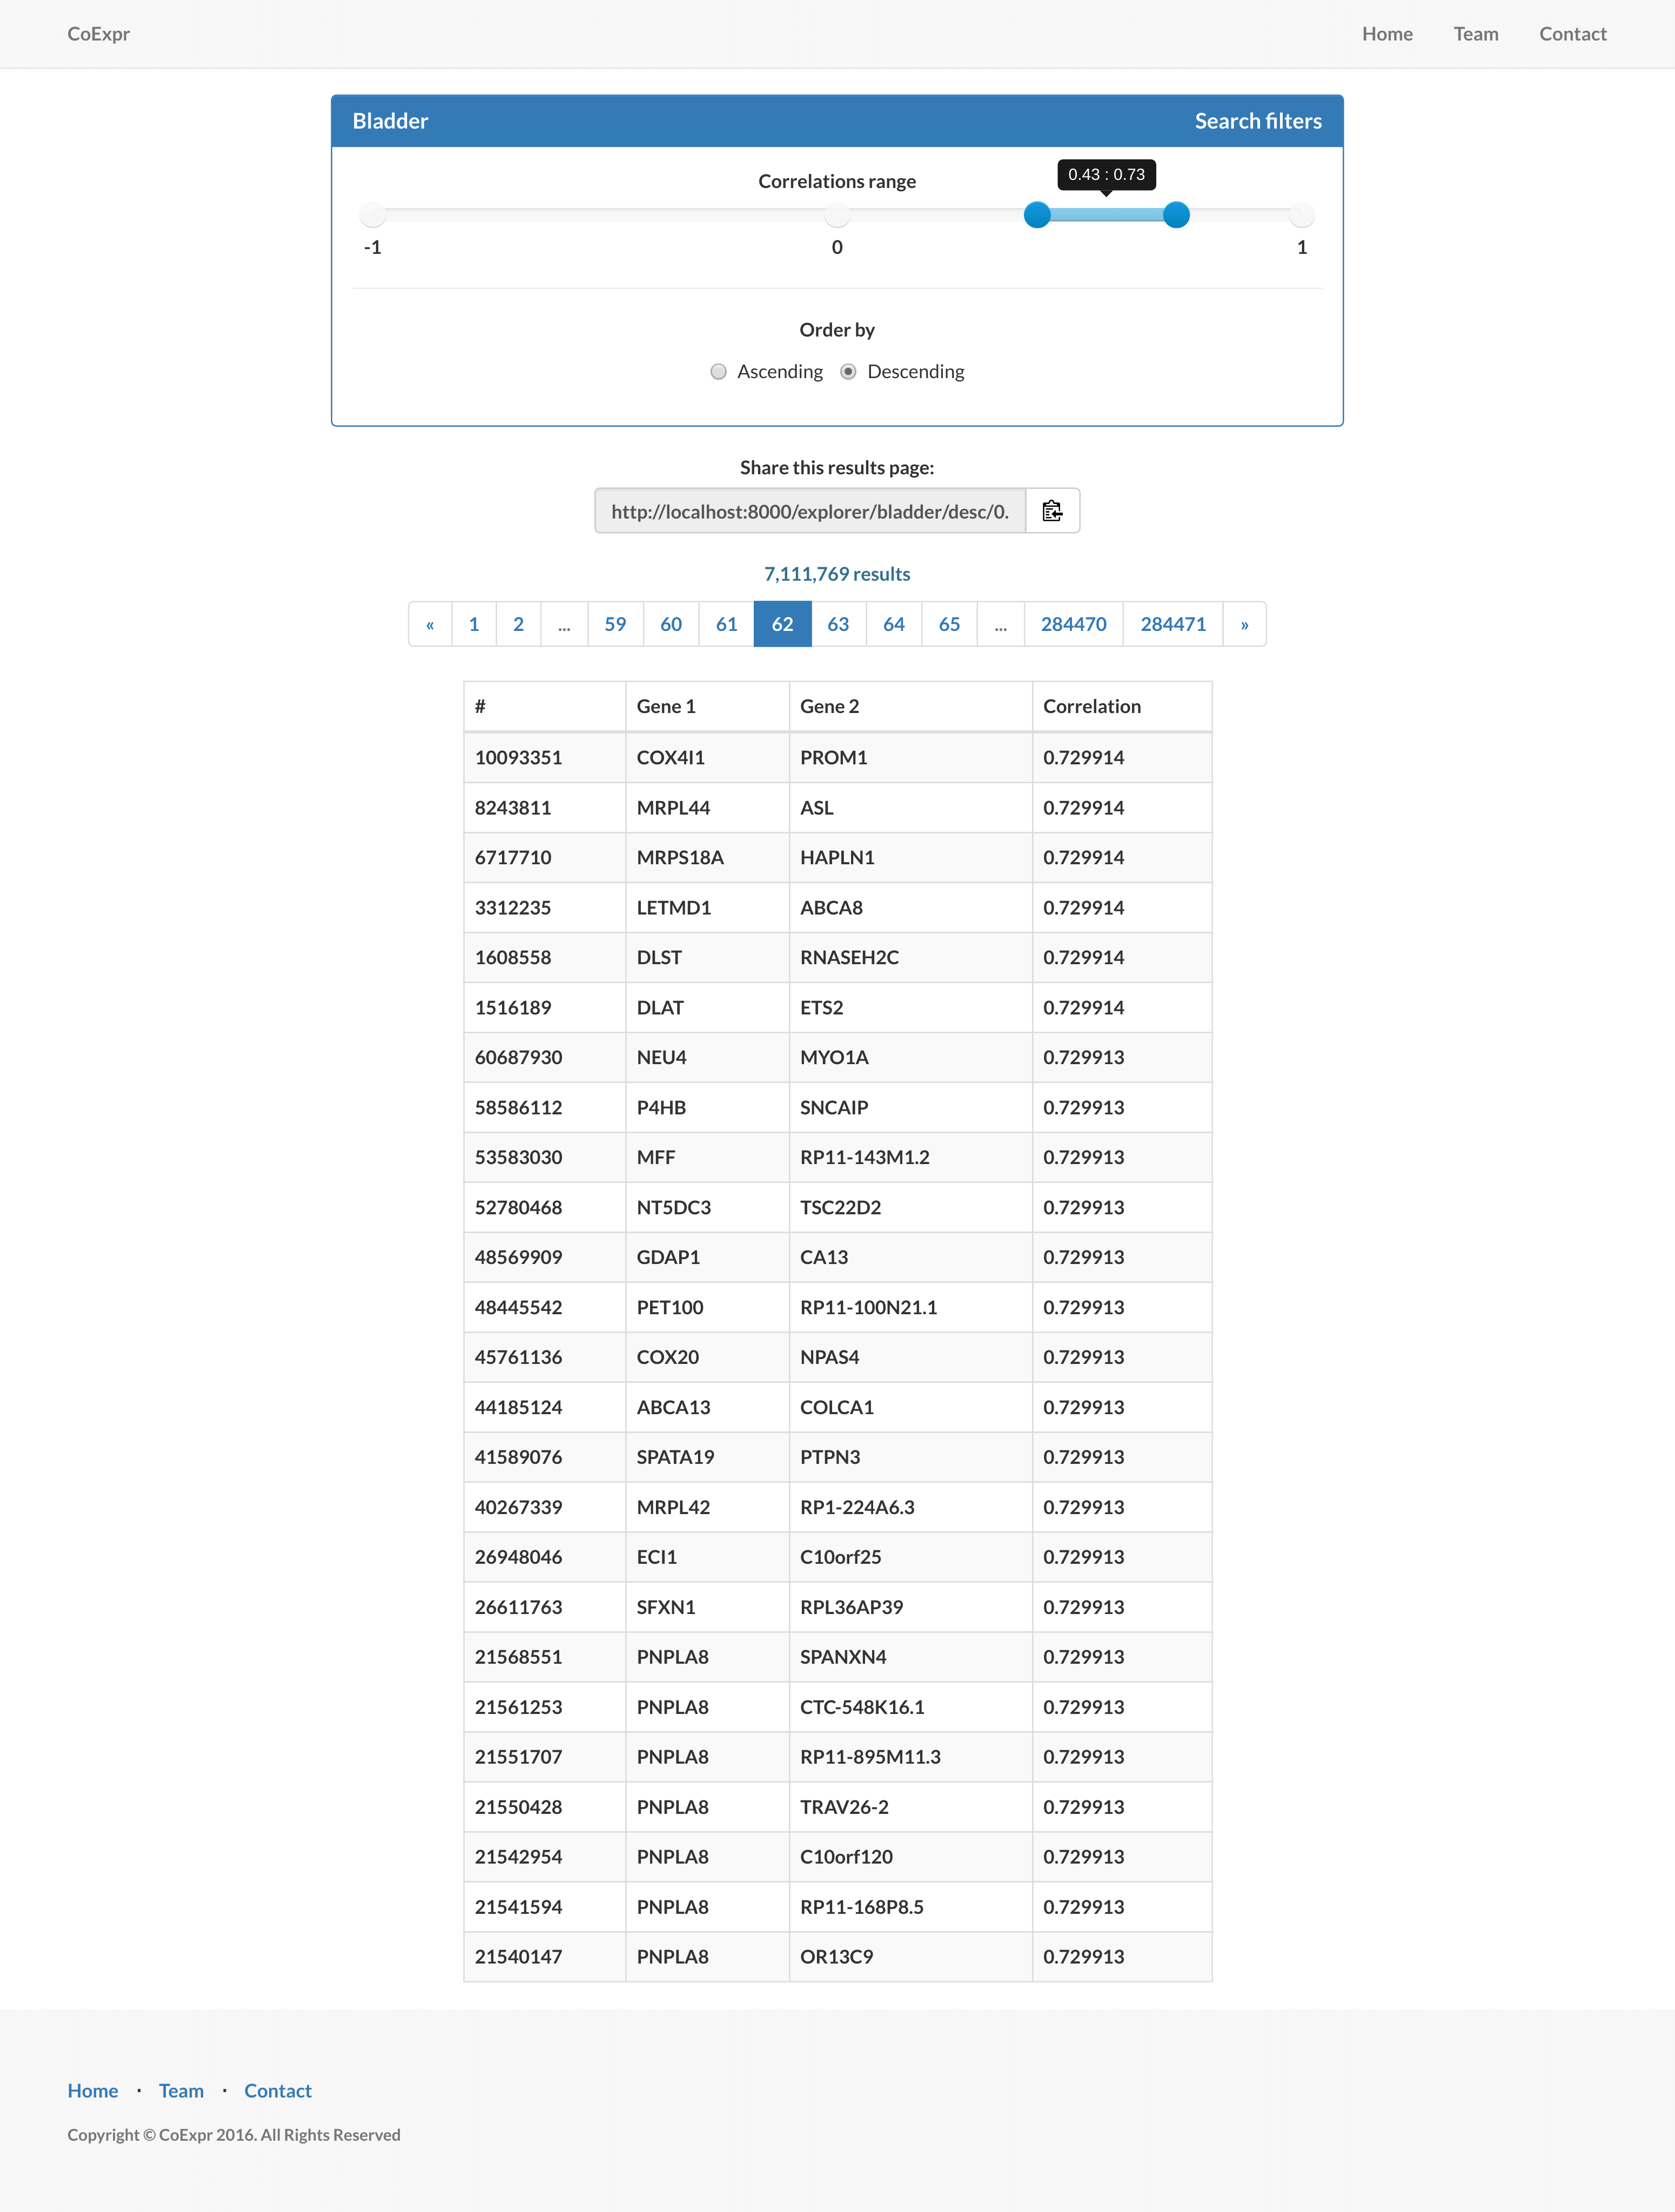
\includegraphics[width=1\linewidth]{res/tissue.png}
    \caption{Página de exploração de um tecido (neste caso da bexiga). O painel, no topo, permite refinar os resultados da pesquisa. Diretamente abaixo do painel encontra-se uma widget para copiar para o clipboard o link dos resultados da pesquisa atual. Finalmente, a tabela mostra os resultados da pesquisa: o ID do par de genes na base de dados, cada um dos genes do par, e a semelhança desses genes.}
    \label{fig:tissuePage}
\end{figure}
